\documentclass[conference]{IEEEtran}
\usepackage{cite}
\usepackage{amsmath,amssymb,amsfonts}
\usepackage{graphicx}
\usepackage{textcomp}
\usepackage{xcolor}
\usepackage{booktabs}
\usepackage{tikz}
\usetikzlibrary{positioning,arrows.meta,calc,backgrounds}
\usepackage{hyperref}

% ---------- placeholder marker (search for \todo before submitting) ----------
\newcommand{\todo}[1]{\textcolor{red}{[TODO: #1]}}

% ---------- macros for the DAgger section ----------
\newcommand{\dagE}{\mathcal{E}}                        % expert
\newcommand{\dagPi}{\pi_\theta}                        % learner policy
\newcommand{\dagD}{\mathcal{D}}                        % dataset
\newcommand{\dagnorm}[1]{\lVert #1\rVert_2}            % Euclidean norm
\newcommand{\dagwrap}{\operatorname{wrap}}             % angle wrapping
\newcommand{\dagNm}{\mathrm{N\!\cdot\!m}}              % newton-metre
\newcommand{\dagone}{\mathbf{1}}                       % indicator
\newcommand{\dagfigdir}{figures/}                      % figure folder

\definecolor{dagblue}{HTML}{1F4E79}
\definecolor{dagblueL}{HTML}{E8F0F8}
\definecolor{daggreen}{HTML}{2E7D32}
\definecolor{daggreenL}{HTML}{E6F4E8}
\definecolor{dagorange}{HTML}{C26A00}
\definecolor{dagorangeL}{HTML}{FFF1DC}
\newcommand{\dagbox}[3]{% {frame colour}{fill colour}{content}
  \par\medskip\noindent
  \fcolorbox{#1}{#2}{\begin{minipage}{\dimexpr\linewidth-2\fboxsep-2\fboxrule\relax}%
    \small\setlength{\parskip}{0.3em}#3\end{minipage}}\par\medskip}

\begin{document}

\title{Behaviour Cloning for a Mobile Manipulator:\\COMP0245 Group 10 Submission}

\author{
\IEEEauthorblockN{Shivansh Chaudhary\IEEEauthorrefmark{1}, Ricktho Sarkar\IEEEauthorrefmark{2}, Hafizh Ilham\IEEEauthorrefmark{3}}
\IEEEauthorblockA{Department of Computer Science, University College London, London, United Kingdom\\
Student IDs: \IEEEauthorrefmark{1}26088192, \IEEEauthorrefmark{2}\todo{ID}, \IEEEauthorrefmark{3}\todo{ID}}
}

\maketitle

\begin{abstract}
This is the Group 10 submission for the COMP0245 lab, in which a model is trained to imitate an expert controller that drives a mobile robot across a room and then reaches a 3D target with its attached arm. The paper presents the data analysis and feature engineering carried out by the group and compares the behaviour-cloning models developed by its members. Three approaches are followed: (i)~a decoupled linear regression model, with one model controlling the base and one controlling the arm; (ii)~a multi-layer perceptron (MLP) policy on egocentric features whose wheel and arm networks are trained with Dataset Aggregation (DAgger); and (iii)~a random forest approach that pairs a random forest base controller, using goal-relative input features, with either a random forest arm or the DAgger-trained MLP arm.

On 1,000 randomised test trials, the decoupled linear model succeeds in 100\% of trials with an average error of 6.3\,mm and an inference time of 0.03\,ms per step. On the same 1,000 trials, the DAgger MLP policy succeeds in 90.0\% of trials from arbitrary spawn poses, with a median error of 18.0\,mm and an inference time of 0.21\,ms per step. On 100 held-out targets, the random forest base with the DAgger MLP arm succeeds in 97\% of trials within 5\,cm (34\% within 1\,cm), while a fully random forest controller fails in every trial despite an offline $R^2$ of up to 0.95.
\end{abstract}

\begin{IEEEkeywords}
Mobile manipulation, behaviour cloning, imitation learning, DAgger, linear regression, random forest, multi-layer perceptron.
\end{IEEEkeywords}

% =========================================================================
% SECTION I: INTRODUCTION
% =========================================================================
\section{Introduction}

\subsection{The Task}
The goal of this assignment is to control a simulated mobile manipulator in PyBullet \cite{coumans2016pybullet}. The robot consists of a Robotnik mobile base with four skid-steer wheels and a 7-DOF Kinova robotic arm.

Given a 3D target position $\mathbf{x}_{\text{target}} = [x_t, y_t, z_t]^T$ placed anywhere in space, the robot must:
\begin{enumerate}
    \item drive its wheels to bring the base close to the target;
    \item stop the base and move its arm so that the gripper reaches the target within a tolerance of $0.05\,\text{m}$ (with $0.01\,\text{m}$ as the ideal goal).
\end{enumerate}
A model is trained on many expert trajectories so that it replicates this behaviour. The input to the model is the robot's current state (base position, heading, arm joint angles and velocities) plus the target; the output is the motor commands: 4 wheel velocities for the base and 7 joint torques for the arm.

\subsection{Robot Constraints and Assumptions}
The following assumptions were made while training the models:
\begin{itemize}
    \item \textbf{Wheels:} 4 skid-steer wheels of radius $0.11\,\text{m}$. The expert caps the forward speed at $v_{\max} = 0.25\,\text{m/s}$ (about $2.27\,\text{rad/s}$ wheel speed), and wheel commands are clipped to $\pm 3.18\,\text{rad/s}$ at execution.
    \item \textbf{Arm joints:} 7 joints with a torque limit of $\pm 30\,\text{N}\cdot\text{m}$. Shoulder Joint~2 ($q_5$) cannot go below $0.82\,\text{rad}$.
    \item \textbf{Environment:} The floor is flat and there are no obstacles between the robot and the target. A solution for the case with obstacles, using the ROS2 Nav2 packages as the global planner and our trained models as local planners, was also explored (Section~\ref{sec:limitations}).
\end{itemize}

% =========================================================================
% SECTION II: DATA ANALYSIS
% =========================================================================
\section{Data Analysis: Why a Naive Input--Output Model Fails}
\label{sec:analysis}

\subsection{Naive Linear Regression}
The first approach was a single linear regression model predicting all 11 motor outputs from all state features at once. In simulation this failed immediately: as soon as the arm moved, it slammed down into the metal base, the physics simulation became unstable, and the robot was launched into the air.

To understand the failure, the raw CSV data were analysed before any further models were trained. The Pearson correlation coefficient ($r \in [-1, 1]$) was computed between all candidate input features and the motor outputs (Fig.~\ref{fig:correlation}). The 4 wheel commands were converted into forward and turning components using differential-drive kinematics \cite{siegwart2011autonomous}:
\begin{equation}
\text{wheel\_fwd} = \frac{\omega_R + \omega_L}{2}, \qquad \text{wheel\_turn} = \frac{\omega_R - \omega_L}{2}.
\end{equation}
The correlation analysis revealed four main findings:
\begin{itemize}
    \item \textbf{World coordinates are uninformative:} the world-frame offsets $\Delta x$ and $\Delta y$ had $r = -0.01$ with forward speed and $r = +0.02$ with turning.
    \item \textbf{Body-frame coordinates are informative:} after rotating into the robot's body frame, \texttt{goal\_forward} rose to $r = +0.51$ with forward speed ($r = +0.79$ when the robot is aligned with the goal), while \texttt{goal\_left} and \texttt{target\_left} rose to $r = +0.81$ and $r = +0.83$ with turning.
    \item \textbf{Heading and bearing drive steering:} \texttt{heading\_error} ($r = +0.61$) and \texttt{bearing\_error} ($r = +0.73$) had clean linear relationships with wheel turning.
    \item \textbf{Spurious correlations from regime mixing:} Shoulder Joint~2 (\texttt{q\_mes\_5}) showed a spurious correlation of $r = +0.34$ with forward wheel speed, only because the arm is locked during driving and moves only during reaching.
\end{itemize}

\begin{figure}[t]
\centering
\includegraphics[width=\columnwidth]{figures/correlation_heatmap.png}
\caption{Pearson correlation heatmap across raw state inputs and motor outputs.}
\label{fig:correlation}
\end{figure}

\begin{figure}[t]
\centering
\includegraphics[width=\columnwidth]{figures/failure_1_regime_mixing.png}
\caption{Regime mixing: the 77.4\% of rows in which the arm is locked flatten the fitted reaching slope from 1.64 to 0.49.}
\label{fig:regime_mixing}
\end{figure}

\subsubsection{Problem 1: Two Different Tasks in One Dataset (Regime Mixing)}
In the expert data the task is split into two separate phases: \textbf{Phase~1 (base driving)}, in which the wheels drive to a parking spot while the arm is locked at its home pose (\textbf{77.4\% of all rows}), and \textbf{Phase~2 (arm reaching)}, in which the wheels are stopped ($0\,\text{rad/s}$) and only the arm moves toward the target (\textbf{22.6\% of rows}).
In 77.4\% of the rows the arm ignores the target because it is locked, which reduces the slope of the fitted reaching model by more than $3\times$ (from $1.64$ to $0.49$, Fig.~\ref{fig:regime_mixing}). The model also learns spurious couplings between the arm torques and the wheel speed, so the arm starts swinging while the target is still metres away.

\begin{figure}[t]
\centering
\includegraphics[width=\columnwidth]{figures/failure_2_world_vs_body.png}
\caption{World coordinates flip sign depending on the robot's orientation ($r=-0.01$). Rotating into the robot's body frame recovers a strong linear relationship ($r=+0.79$ when aligned).}
\label{fig:world_vs_body}
\end{figure}

\subsubsection{Problem 2: World Coordinates Flip Sign When the Robot Turns}
If a target is 1\,m in front of the robot, it lies at $\Delta x = +1.0\,\text{m}$ when the robot faces East ($\psi = 0^\circ$) but at $\Delta x = -1.0\,\text{m}$ when it faces West ($\psi = 180^\circ$). Because world coordinates flip sign with the robot's heading, wheel speed plotted against world $\Delta x$ shows no correlation ($r = -0.01$, Fig.~\ref{fig:world_vs_body}).
Rotating the target offset into the robot's body frame,
\begin{equation}
\begin{bmatrix} t_f \\ t_l \end{bmatrix} = \begin{bmatrix} \cos\psi & \sin\psi \\ -\sin\psi & \cos\psi \end{bmatrix} \begin{bmatrix} x_t - x_b \\ y_t - y_b \end{bmatrix},
\end{equation}
where $(x_b, y_b)$ is the base position and $t_f$, $t_l$ are the forward and leftward offsets, gives a strong linear relationship ($r = +0.79$ when aligned).

\begin{figure}[t]
\centering
\includegraphics[width=\columnwidth]{figures/failure_3_positive_feedback.png}
\caption{The anti-spring instability. (A)~Learned joint-angle weights with collinear inputs (red) and after the fixes of Section~\ref{sec:linear} (green). (B)~The resulting runaway of the shoulder joint.}
\label{fig:positive_feedback}
\end{figure}

\subsubsection{Problem 3: The ``Anti-Spring'' Instability}
The original feature list included both the joint angles $q$ and the gripper position $\mathbf{x}_{\text{ee}}$. The gripper position is fully determined by the joint angles ($\mathbf{x}_{\text{ee}} = f(q)$), so the two are strongly collinear. Linear regression suffered from this multicollinearity: it assigned a negative weight to the gripper position and a \textbf{positive weight to the shoulder joint angle} ($+11.1\,\text{N}\cdot\text{m/rad}$ on Joint~2, Fig.~\ref{fig:positive_feedback}A).
A stabilising spring applies a restoring torque $-kq$ with $k > 0$, i.e.\ a \emph{negative} weight on $q$, which opposes any deviation. A positive weight is an \textbf{anti-spring}: when gravity pulls the shoulder down, the controller pushes it down \emph{harder}, creating an exponential runaway (Fig.~\ref{fig:positive_feedback}B) that slams the arm into the chassis.

\begin{figure}[t]
\centering
\includegraphics[width=\columnwidth]{figures/failure_4_data_and_ik_branching.png}
\caption{Elbow-twist bifurcation at low target heights.}
\label{fig:ik_branching}
\end{figure}

\subsubsection{Problem 4: Saturated Joints and the Elbow-Twist Bifurcation}
For targets above $z = 0.46\,\text{m}$ the arm reaches normally. At $z = 0.46\,\text{m}$, however, Shoulder Joint~2 reaches the lowest value the expert commands ($0.87\,\text{rad}$, i.e.\ $0.05\,\text{rad}$ inside its $0.82\,\text{rad}$ limit) and stays there (Fig.~\ref{fig:ik_branching}B).
To reach lower ($z \le 0.46\,\text{m}$), the expert twists the elbow roll joint ($q_6$) either to the left ($+0.55\,\text{rad}$) or to the right ($-0.60\,\text{rad}$) with roughly equal probability. Trained on both branches, a least-squares regressor predicts their average, $(+0.55 - 0.60)/2 \approx \mathbf{0.0\,\text{rad}}$ \cite{bishop1994mixture}, so the arm tries to reach straight down without twisting the elbow and gets stuck.

\subsection{Final Feature Sets for the Base and Arm}
\label{sec:features}
Based on these findings, the following feature sets were chosen for the linear regression models:
\begin{itemize}
    \item \textbf{Base model (15 features)}, engineered from the body-frame goal offsets $(g_f, g_l)$, the distance $d = \sqrt{g_f^2 + g_l^2}$, the heading error $\theta_{\text{head}}$ and the parking bearing error $\theta_{\text{bear}}$:
    \begin{enumerate}
        \item Saturated offsets: $g_f$ and $g_l$ clipped to $[-0.35, 0.35]\,\text{m}$.
        \item Saturated distance: $d_{\text{sat}} = \min(d, 0.35\,\text{m})$, which prevents overspeeding on far targets.
        \item Alignment gate: $\text{aligned} = \max(0, \cos\theta_{\text{head}} - 0.85)$.
        \item Drive term: $\text{drive\_term} = \max(0, d_{\text{sat}} - 0.04) \cdot \text{aligned}$, which blocks forward driving until the robot points at the goal.
        \item Blending weights: $\text{near\_goal} = \text{clip}\bigl((0.12 - d)/0.12, 0, 1\bigr)$ and $\text{far\_goal} = 1 - \text{near\_goal}$.
        \item Far steering (4 features): $\text{far\_goal} \times [\theta_{\text{head}}, \sin\theta_{\text{head}}, |\theta_{\text{head}}|]$ and $\cos\theta_{\text{head}}$.
        \item Near docking (5 features): $\text{near\_goal} \times [\theta_{\text{bear}}, \sin\theta_{\text{bear}}, |\theta_{\text{bear}}|]$, the raw $\theta_{\text{bear}}$, and $\cos\theta_{\text{bear}}$.
    \end{enumerate}
    \todo{the items above list 16 quantities; check which one is not a separate feature, or change the count to 16}
    \item \textbf{Arm model (25 features)}, designed to learn stabilising PD spring--damper control and the low-height elbow twist:
    \begin{enumerate}
        \item 7 measured joint positions $q_{\text{mes},4..10}$ ($\mathbf{x}_{\text{ee}}$ is omitted to remove the anti-spring effect).
        \item 7 measured joint velocities $\dot{q}_{\text{mes},4..10}$ (to learn the damping term $-K_d \dot{q}$).
        \item 3 body-frame target offsets $(t_f, t_l, t_h)$ from the robot base to the target.
        \item 6 quadratic cross terms $t_f^2, t_l^2, t_h^2, t_f t_h, t_f t_l, t_l t_h$ (to fit the curvature of the arm workspace).
        \item 2 low-height hinge features, $\text{low\_z} = \max(0, 0.46 - t_h)$ and $\text{low\_z}^2$ (to command the positive elbow twist once Shoulder Joint~2 saturates).
    \end{enumerate}
\end{itemize}

% TODO (Ricktho / Hafizh): add any further data analysis here.

% =========================================================================
% SECTION III: METHODOLOGY
% =========================================================================
\section{Methodology}
\label{sec:method}

The team compared three approaches:
\begin{enumerate}
    \item a \textbf{decoupled linear regression} model with hand-engineered physical basis functions (Shivansh Chaudhary, Section~\ref{sec:linear});
    \item an \textbf{MLP policy trained with DAgger} (Ricktho Sarkar, Section~\ref{dag:sec});
    \item a \textbf{random forest} controller, combined with either a random forest arm or the DAgger MLP arm (Hafizh Ilham, Section~\ref{sec:rf}).
\end{enumerate}

\subsection{Approach 1: Decoupled Linear Regression}
\label{sec:linear}
Instead of forcing one model to do everything, two independent linear models were trained.

\subsubsection{Mobile Base Model (Phase 1)}
The base only needs to drive to a parking spot roughly $0.70\,\text{m}$ in front of the target. For this, the 15-feature linear model of Section~\ref{sec:features} mapping to the 4 wheel speeds was developed. Two features are key:
\begin{itemize}
    \item \textbf{Distance saturation:} if a target is 5\,m away, the raw distance would command five times more speed than anything seen in training. Saturating the distance at $0.35\,\text{m}$ ($d_{\text{sat}} = \min(d, 0.35)$) lets the robot drive safely to arbitrarily distant targets.
    \item \textbf{Alignment gate (\texttt{drive\_term}):} the robot should not drive forward unless it faces the goal. In a purely linear model ($w_1 d - w_2 \theta$), a large distance still pushes the robot forward even when it faces away. An interaction feature prevents this:
    \begin{equation}
    \begin{aligned}
    \text{drive\_term} = {}&\max(0,\, d_{\text{sat}} - 0.04)\\
    &\cdot \max(0,\, \cos\theta_{\text{head}} - 0.85).
    \end{aligned}
    \end{equation}
    If the heading error exceeds $31.8^\circ$ ($\cos\theta_{\text{head}} < 0.85$), this term is exactly zero, so the wheels can only turn the robot in place until it points at the goal.
\end{itemize}

\subsubsection{Arm Torque Model (Phase 2)}
From control theory \cite{takegaki1981new}, the ideal arm torque is
\begin{equation}
\boldsymbol{\tau}^* = \boldsymbol{\tau}_g(q_{\text{final}}) + K_p(q_{\text{final}} - q) - K_d \dot{q},
\end{equation}
which has three parts: gravity compensation, a spring pulling the arm to the target pose, and a damper suppressing oscillations.

To let linear regression learn this law without falling into the anti-spring trap:
\begin{enumerate}
    \item the gripper position $\mathbf{x}_{\text{ee}}$ was removed from the inputs;
    \item failed timeout episodes ($2.8\%$ of the data) were removed, and low-height episodes on the negative elbow branch were filtered out, keeping only the positive elbow-twist branch ($q_6 \ge +0.2\,\text{rad}$);
    \item the hinge term $\text{low\_z} = \max(0, 0.46 - t_h)$ was added so that the model can twist the elbow roll joint specifically for low targets;
    \item \textbf{DART noise injection \cite{laskey2017dart}:} in clean expert data the arm is never pushed off course, so the model never learns which restoring torque to apply. Small random perturbations were therefore applied to the joint angles ($\delta q \sim \mathcal{N}(0, 0.08^2)$) and velocities ($\delta \dot{q} \sim \mathcal{N}(0, 0.15^2)$), and the model was trained on the expert's restoring torque.
\end{enumerate}
With these changes, linear regression recovered the expert's spring stiffness of $-100\,\text{N}\cdot\text{m/rad}$ on all 7 joints (Fig.~\ref{fig:positive_feedback}A, green bars).

% -------------------------------------------------------------------------
% SUBSECTION B: MLP + DAgger
% -------------------------------------------------------------------------
\subsection{Approach 2: MLP Policy with DAgger}
\label{dag:sec}

In parallel, a Multi-Layer Perceptron (MLP) policy was developed in PyTorch to test whether neural networks can learn the complete behaviour (driving \emph{and} reaching) from lightly processed features, using Dataset Aggregation (DAgger) \cite{ross2011reduction} to remove the compounding errors of plain behaviour cloning. The final policy (V6) is the result of six iterations; Section~\ref{dag:history} summarises how it was reached.

\subsubsection{Problem and Key Idea}
\label{dag:problem}

The robot must (i)~drive its four-wheel base to a standoff pose in front of a world-frame target and then (ii)~move its 7-joint arm so that the end-effector reaches the target and stays there. PyBullet simulates the physics and Pinocchio provides kinematics and dynamics. At step $t$ the robot is in state $s_t$ and receives a command $a_t=[u_{wheel},u_{arm}]$, where $u_{wheel}\in\mathbb{R}^4$ are wheel angular velocities (rad/s) and $u_{arm}\in\mathbb{R}^7$ are joint torques ($\dagNm$). A learned policy $\dagPi$ with weights $\theta$ imitates a model-based \emph{expert controller} $\dagE$:
\begin{equation}
  \dagPi\bigl(\phi(s_t)\bigr)\;\approx\;a_t^{*}=\dagE(s_t),
  \label{dag:goal}
\end{equation}
where $\phi(s_t)$ is a fixed-length feature vector (Section~\ref{dag:state}); we write $\dagPi(s_t)$ for $\dagPi(\phi(s_t))$.

Training only on states the expert visits (\emph{behaviour cloning}, BC) is not enough: a small learner error leads to a state the expert never visited, where the network errs more, so the errors \emph{compound}. For a horizon of $T$ steps and a per-step imitation error $\epsilon$, BC can accumulate $O(T^{2}\epsilon)$ cost, whereas DAgger achieves $O(T\epsilon)$ \cite{ross2011reduction}, because it trains on the states that the learner itself reaches. The horizon here is long: a typical episode lasts 10--20\,s, i.e.\ $T=10^4$--$2\cdot10^4$ control steps of 1\,ms.

\dagbox{dagblue}{dagblueL}{%
\textbf{Key idea of DAgger (Dataset Aggregation).} Let the \emph{learner} drive, ask the \emph{expert} what it would have done in every state the learner actually reaches, add these expert-labelled states to the training set, and retrain.}

In V6 \emph{all three} networks (wheels, arm HOLD, arm REACH) are trained with DAgger, so the guarantee above applies to the complete policy. The notation is summarised in Table~\ref{dag:tab:notation}.

\begin{table}[t]
\caption{Notation for the DAgger Pipeline}
\label{dag:tab:notation}
\centering
\footnotesize
\renewcommand{\arraystretch}{1.12}
\begin{tabular}{@{}p{2.5cm}p{5.7cm}@{}}
\toprule
\textbf{Symbol} & \textbf{Meaning}\\
\midrule
$s_t,\ \phi(s_t)$ & robot state and its 38-dimensional egocentric feature vector\\
$\phi_{arm}(t)$ & 66-dimensional arm input: $\phi(s_t)$ plus the joint state 10\,ms and 30\,ms earlier\\
$a_t,\ a_t^{*}$ & executed and expert (label) action, $\in\mathbb{R}^4\times\mathbb{R}^7$\\
$\dagE,\ \dagPi$ & expert controller; learner policy with weights $\theta$\\
$\beta,\ M$ & probability of expert control per mixing interval; interval length in steps\\
$\dagD_k$ & aggregated dataset after DAgger round $k$\\
$d_{\dagPi}$ & state distribution induced by running $\dagPi$\\
$p_{base},\ \psi$ & base position and yaw\\
$p_{goal},\ \theta_{goal}$ & base goal position and goal bearing (derived from the target)\\
$p_{ee},\ p_{target}$ & end-effector position and world-frame target\\
$d,\ \Delta\theta_{head},\ \Delta\theta_{ori}$ & distance to goal, heading error toward the goal, final orientation error\\
$c_t,\ \hat c_t$ & raw and latched navigation-complete flags\\
$q,\ \dot q,\ q_{init}$ & arm joint angles, velocities (7 joints) and initial arm configuration\\
$q_{des},\ \dot q_{des}$ & desired joint angles and velocities (expert reference)\\
$J,\ v_{cart},\ \lambda$ & end-effector Jacobian ($3\times7$), desired Cartesian velocity, IK damping\\
$K_p,\ K_d,\ g(q)$ & PD gains and gravity-compensation torque\\
\bottomrule
\end{tabular}
\end{table}

\subsubsection{Task Geometry}
\label{dag:geom-sec}

\paragraph{Base goal} The target $p_{target}\in\mathbb{R}^3$ is given in the world frame. The base is sent to a \emph{standoff} pose on the ray from the world origin through the target's $xy$-position:
\begin{equation}
\begin{aligned}
  \theta_{goal}&=\operatorname{atan2}(p_{target,y},\,p_{target,x}),\\
  p_{goal}&=p_{target,xy}-\sigma(p_{target,z})\begin{bmatrix}\cos\theta_{goal}\\ \sin\theta_{goal}\end{bmatrix},
\end{aligned}
\label{dag:goalpose}
\end{equation}
where the standoff distance $\sigma(z)$ interpolates $(z,\sigma)=(0.1,0.80),(0.5,0.65),(1.1,0.65),(1.25,0.35)$\,m: higher targets are approached more closely.

\paragraph{Navigation signals} From the base pose,
\begin{equation}
\begin{aligned}
  \Delta p&=p_{goal}-p_{base},\qquad d=\dagnorm{\Delta p},\\
  \Delta\theta_{head}&=\dagwrap\bigl(\operatorname{atan2}(\Delta p_y,\Delta p_x)-\psi\bigr),\\
  \Delta\theta_{ori}&=\dagwrap(\theta_{goal}-\psi),
\end{aligned}
\label{dag:geom}
\end{equation}
where $\dagwrap(\cdot)$ maps an angle to $(-\pi,\pi]$. $\Delta\theta_{head}$ is how far the base must turn to \emph{face the goal point} and $\Delta\theta_{ori}$ how far it must turn to reach the final \emph{orientation}. The observable \emph{navigation-complete} flag is
\begin{equation}
  c_t=\dagone\bigl[(d<0.08\,\text{m}\wedge|\Delta\theta_{ori}|<0.05\,\text{rad})\vee t>t_{nav}\bigr],
\label{dag:nav}
\end{equation}
with a navigation timeout $t_{nav}=45$\,s. The timeout was raised from 25\,s because drives from a spawn 4\,m away take up to $\approx 30$\,s at the expert's 0.25\,m/s cap.

\subsubsection{Expert Controller}
\label{dag:expert}

The expert is \emph{stateful}: the base keeps a phase variable and the arm keeps its reference $q_{des}$, so $a_t^{*}=\dagE(s_t;z_t)$ with internal state $z_t=(\text{base phase},q_{des})$. To keep $z_t$ consistent, the collector advances the expert on \emph{every} observed state, including steps in which the learner acts. The expert was left unchanged in all versions; it succeeded in 18/18 test episodes from spawns up to 2\,m away, so it is a valid teacher for the wide-spawn task.

\paragraph{Base (skid-steer)} The phases are \emph{align}~$\to$~\emph{drive}~$\to$~\emph{orient}~$\to$~\emph{done}:
\begin{itemize}
  \item \emph{align}: turn in place with $\omega=\operatorname{clip}(3\,\Delta\theta_{head},\pm1.0)$\,rad/s until $|\Delta\theta_{head}|<0.05$ (or $d<0.08$);
  \item \emph{drive}: $v=\operatorname{clip}(1.0\,d,\,0.05,\,0.25)\cdot\max(0,\cos\Delta\theta_{head})$\,m/s with steering $\omega=\operatorname{clip}(1.5\,\Delta\theta_{head},\pm0.3)$\,rad/s, until $d<0.08$ or the goal has been passed ($d<0.15$ and $\cos\Delta\theta_{head}<0$);
  \item \emph{orient}: $\omega=\operatorname{clip}(3\,\Delta\theta_{ori},\pm1.0)$ until $|\Delta\theta_{ori}|<0.05$; then \emph{done} (wheels held at zero). The timeout $t_{nav}$ also sets \emph{done}.
\end{itemize}
$(v,\omega)$ is converted to wheel speeds $\omega_{L,R}=(v\mp\omega B/2)/r$ with wheel radius $r=0.11$\,m and effective track width $B=0.66$\,m, ordered $[\omega_R,\omega_L,\omega_L,\omega_R]$ and clipped to $\pm3.18$\,rad/s.

\paragraph{Arm: two modes} While the base is not done, the arm \emph{holds} its initial configuration: $q_{des}=q_{init}$, $\dot q_{des}=0$. Once the base is done, the arm \emph{reaches}: the target is clamped to a sphere of radius $0.85$\,m around the shoulder (giving $p'_{target}$), and a proportional Cartesian velocity with capped norm is commanded,
\begin{equation}
  v_{cart}=\operatorname{clip}_{\lVert\cdot\rVert\le0.25\,\text{m/s}}\bigl(1.5\,(p'_{target}-p_{ee})\bigr).
  \label{dag:vcart}
\end{equation}
Since $J\in\mathbb{R}^{3\times7}$ is not square and loses rank near singular poses, the joint velocity solves a \emph{damped least-squares} problem:
\begin{equation}
\begin{aligned}
  \dot q_{des}&=\arg\min_{\dot q}\ \dagnorm{J\dot q-v_{cart}}^{2}+\lambda^{2}\dagnorm{\dot q}^{2}\\
  &=J^{\top}\bigl(JJ^{\top}+\lambda^{2}I_3\bigr)^{-1}v_{cart}.
\end{aligned}
\label{dag:dls}
\end{equation}
The closed form follows from $(J^{\top}J+\lambda^{2}I)\dot q=J^{\top}v_{cart}$ and the identity $(J^{\top}J+\lambda^{2}I)^{-1}J^{\top}=J^{\top}(JJ^{\top}+\lambda^{2}I)^{-1}$. The damping is interpolated from $0.10$ (at $\sigma_{\min}(J)=0$) to $0.01$ (at $\sigma_{\min}\ge0.15$), so it is large only near singularities. Joints within $0.05$\,rad of a limit that the solution would push further are frozen and \eqref{dag:dls} is re-solved (up to 7 passes). The result is scaled to $\max_j|\dot q_{des,j}|\le1.0$\,rad/s and the reference is integrated and clipped,
\begin{equation}
  q_{des}\leftarrow\operatorname{clip}_{[q-q_{lead},\,q+q_{lead}]}\bigl(q_{des}+\dot q_{des}\Delta t\bigr),\quad q_{lead}=0.15\,\text{rad},
\label{dag:qlead}
\end{equation}
and kept $0.05$\,rad inside the joint limits. The window $q_{lead}$ is an anti-windup measure: for an unreachable target the reference cannot run away from the arm.

\paragraph{Torque law} In both modes a PD law with gravity compensation produces the torques,
\begin{equation}
  \tau_{arm}=\operatorname{clip}_{[-30,30]\,\dagNm}\Bigl(K_p(q_{des}-q)+K_d(\dot q_{des}-\dot q)+g(q)\Bigr),
  \label{dag:pd}
\end{equation}
with $K_p=100$ and $K_d=30$: a spring toward $q_{des}$, a damper, and gravity cancellation $g(q)$ from the Pinocchio model, the same structure that the linear arm model of Section~\ref{sec:linear} recovers. The fingers are held at $0.1$\,rad by position control and are not part of the policy.

\subsubsection{Egocentric State Features}
\label{dag:state}

Every rollout logs the same 38 raw quantities (base pose, target, end-effector, goal, $q$, $\dot q$, $q_{init}$, the navigation signals and $c_t$). The networks do not see them directly; they see the \emph{egocentric} transformation, in which every position is expressed in the robot's base frame (forward $f$, left $l$, up $u$):
\begin{equation}
  \begin{bmatrix} f\\ l\end{bmatrix}=\begin{bmatrix}\cos\psi&\sin\psi\\-\sin\psi&\cos\psi\end{bmatrix}\bigl(p_{xy}-p_{base,xy}\bigr),\quad u=p_z-p_{base,z}.
  \label{dag:ego}
\end{equation}
The 38 network inputs are: the goal $(f,l)$ (2); the target $(f,l,u)$ (3); the end-effector $(f,l,u)$ (3); the reaching error $p_{target}-p_{ee}$ in the base frame (3); $d$ (1); $\sin$ and $\cos$ of $\Delta\theta_{head}$ and of $\Delta\theta_{ori}$ (4); $q$, $\dot q$ and $q_{init}$ (21); and the latched flag $\hat c_t$ (1). The reasons for each choice are:
\begin{itemize}
  \item \textbf{Base frame.} The correct command depends only on where the goal and target are \emph{relative to the robot}. This is the same finding as Problem~2 of Section~\ref{sec:analysis} ($r=-0.01$ in world coordinates versus $r=+0.79$ in the body frame). With Eq.~\eqref{dag:ego} the inputs are invariant to translations and rotations of the whole scene, so a network trained on spawns in a $4\times4$\,m square also works for targets and spawns outside it (Section~\ref{dag:results}).
  \item \textbf{Explicit reaching error.} The expert's Cartesian command \eqref{dag:vcart} is proportional to $p'_{target}-p_{ee}$; providing this difference directly saves the network from learning a subtraction of two large, correlated inputs.
  \item \textbf{$\sin/\cos$ of angles.} A raw angle jumps by $2\pi$ at $\pm\pi$ although the physical state is unchanged; $(\sin,\cos)$ is continuous, so nearby states have nearby inputs.
  \item \textbf{$q_{init}$.} In HOLD mode the expert tracks $q_{des}=q_{init}$, so the HOLD network needs it.
  \item \textbf{No scaling.} All inputs are already of order one (metres, radians, rad/s), so no normaliser has to be stored and matched at deployment. A metadata file records the feature and output names, and the loader rejects a checkpoint whose feature contract differs.
\end{itemize}
Only quantities observable at deployment are used; the expert's internal reference $q_{des}$ is logged for diagnosis but \emph{never} given to the learner.

\subsubsection{Learned Policy: Three Networks}
\label{dag:policy}

The deployed policy consists of three MLPs:
\begin{itemize}
  \item a \textbf{wheel network}, $\phi(s_t)\in\mathbb{R}^{38}\to u_{wheel}\in\mathbb{R}^4$;
  \item an \textbf{arm HOLD network} and an \textbf{arm REACH network}, $\phi_{arm}(t)\in\mathbb{R}^{66}\to u_{arm}\in\mathbb{R}^7$.
\end{itemize}
Separate HOLD and REACH networks avoid the regime mixing of Problem~1 in Section~\ref{sec:analysis}: holding a pose and reaching a target are different control laws, and one network fitted to both blurs them. The network is selected by the \emph{latched} flag,
\begin{equation}
  \hat c_t=\max_{\tau\le t}c_\tau,\qquad
  \text{use }\begin{cases}\text{REACH}&\hat c_t=1,\\ \text{HOLD}&\hat c_t=0,\end{cases}
  \label{dag:latch}
\end{equation}
which keeps the phase at 1 once navigation has finished, even if a small base drift later makes the raw flag flicker back to 0. All three networks receive $\hat c_t$, in training and at deployment.

\paragraph{Joint history} The arm input appends the joint state $y=(q,\dot q)\in\mathbb{R}^{14}$ from 10\,ms and 30\,ms earlier,
\begin{equation}
  \phi_{arm}(t)=\bigl[\ \phi(s_t);\ y(t-10\,\text{ms});\ y(t-30\,\text{ms})\ \bigr]\in\mathbb{R}^{38+14+14},
  \label{dag:lags}
\end{equation}
clamped at the start of an episode. The expert is stateful: its reference $q_{des}$ is an integral over the past \eqref{dag:qlead}, so a single snapshot does not determine its action. The short history makes the hidden state partly observable (velocity and acceleration trends), which is what the network needs to reproduce the PD torque \eqref{dag:pd}. The lags are defined in \emph{seconds}: the simulator steps at 1\,ms (10 and 30 steps at deployment), and every training trajectory is resampled to one row per 10\,ms (1 and 3 rows). This gives the history the same physical meaning in training and deployment. Resampling the 1\,ms rollouts also removes nearly duplicate consecutive rows and makes the rollouts match the 10\,ms demonstrations.

\paragraph{Architecture} Each network is
\begin{multline*}
  \mathrm{Lin}(d_{in},256)\to\mathrm{ReLU}\to\mathrm{Drop}(0.1)\\
  \to\mathrm{Lin}(256,256)\to\mathrm{ReLU}\to\mathrm{Drop}(0.1)\\
  \to\mathrm{Lin}(256,128)\to\mathrm{ReLU}\to\mathrm{Drop}(0.1)\\
  \to\mathrm{Lin}(128,d_{out}),
\end{multline*}
where $\mathrm{Lin}(m,n)$ is a fully connected layer $y=Wx+b$, ReLU supplies the nonlinearity needed for the piecewise expert (phase switches, saturations, clipping), and $\mathrm{Drop}(0.1)$ zeroes $10\%$ of the activations during training only, as a mild regulariser. The wheel network has 109\,188 parameters and each arm network 116\,743, i.e.\ 342\,674 in total.

\subsubsection{DAgger Data Collection}
\label{dag:collect}

At every step $t$ of a rollout the loop in Fig.~\ref{dag:fig} runs: (1)~compute $\phi(s_t)$ and the learner action $a_t^{learner}$; (2)~advance the expert and obtain $a_t^{expert}$ in the same state; (3)~execute the action selected by the source setting; (4)~store the \emph{expert} action as the label; (5)~step the simulator. Wheels and arm each have a source $\in\{\text{expert},\text{learner},\text{mix}\}$. In \emph{mix} mode one Bernoulli draw $b_k\sim\mathrm{Bernoulli}(\beta)$ is made every $M$ steps and shared by wheels and arm:
\begin{equation}
  a_t=\begin{cases}a_t^{expert}&\text{if }b_{\lfloor t/M\rfloor}=1,\\ a_t^{learner}&\text{otherwise.}\end{cases}
  \label{dag:mix}
\end{equation}
Holding the choice for $M$ steps lets a learner segment run long enough to drift into realistic error states. After each round the dataset is aggregated,
\begin{equation}
  \dagD_{k+1}=\dagD_{k}\cup\bigl\{(\phi(s_t),\phi_{arm}(t),a_t^{expert}):\ s_t\text{ visited in round }k\bigr\},
\label{dag:agg}
\end{equation}
where $\dagD_0$ holds the 1400 training episodes of the 2000 expert demonstrations (split by episode into 1400/300/300 train/validation/test; the test episodes are never used). The label is \emph{always} the expert's, whichever policy drove the robot, so the supervision stays correct while the learner is in control.

\begin{figure*}[t]
\centering
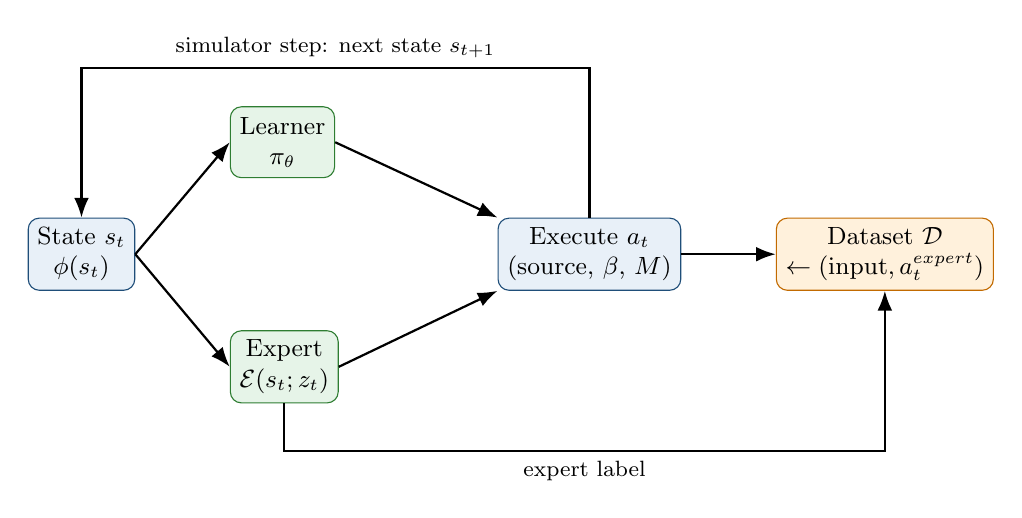
\begin{tikzpicture}[
  box/.style={draw=dagblue, rounded corners, align=center, fill=dagblueL, minimum height=0.9cm, font=\small},
  proc/.style={draw=daggreen, rounded corners, align=center, fill=daggreenL, minimum height=0.9cm, font=\small},
  data/.style={draw=dagorange, rounded corners, align=center, fill=dagorangeL, minimum height=0.9cm, font=\small},
  arr/.style={-{Latex[length=2.5mm]}, thick}]
\node[box]  (s) {State $s_t$\\$\phi(s_t)$};
\node[proc, above right=0.5cm and 1.2cm of s] (l) {Learner\\$\dagPi$};
\node[proc, below right=0.5cm and 1.2cm of s] (e) {Expert\\$\dagE(s_t;z_t)$};
\node[box, right=4.6cm of s] (x) {Execute $a_t$\\(source, $\beta$, $M$)};
\node[data, right=1.2cm of x] (d) {Dataset $\dagD$\\$\leftarrow (\text{input},a_t^{expert})$};
\draw[arr] (s.east)--(l.west);
\draw[arr] (s.east)--(e.west);
\draw[arr] (l.east)--(x.north west);
\draw[arr] (e.east)--(x.south west);
\draw[arr] (x)--(d);
\draw[arr] (e.south) -- ++(0,-0.6) -| node[pos=0.25,below,font=\footnotesize]{expert label} (d.south);
\draw[arr] (x.north) -- ++(0,1.9) -| node[pos=0.25,above,font=\footnotesize]{simulator step: next state $s_{t+1}$} (s.north);
\end{tikzpicture}
\caption{DAgger data collection. Learner and expert are evaluated in the same state (the stateful expert is advanced at every step); the source setting decides which action is executed, and the expert action is always stored as the label.}
\label{dag:fig}
\end{figure*}

\paragraph{Rounds} Table~\ref{dag:tab:rounds} lists the three rounds. Each rollout uses a new random task: the target lies in a uniform direction around the world origin at a horizontal radius of 0.4--1.8\,m and a height of 0.2--1.2\,m; the base spawns uniformly in $x,y\in[-2,2]$\,m with any yaw. Rollouts are logged every 10\,ms and capped at 60\,s. The schedule follows the decaying-$\beta$ recipe of \cite{ross2011reduction}:
\begin{itemize}
  \item \textbf{Round 0} ($\beta=1$, expert only) is behaviour cloning on the \emph{new task distribution}. The 8\,s demonstrations only start within $\pm0.25$\,m of the origin, so they contain no long drives, no large turns and no recoveries; round~0 adds expert coverage of exactly those states.
  \item \textbf{Round 1} ($\beta=0.5$, wheels \emph{and} arm mixed, $M=300$ steps $=0.3$\,s). An immature learner in full control often fails early, and the rest of the rollout is then spent in states that are irrelevant for a good policy. Alternating 0.3\,s segments let the learner drift (up to $7.5$\,cm of travel or $0.3$\,rad of turn per segment) and the expert recover, which yields labels on the ``slightly wrong'' states that matter most.
  \item \textbf{Round 2} ($\beta=0$, learner only) samples $d_{\dagPi}$ itself, the distribution the deployed policy will meet.
\end{itemize}
Wheels are part of the mixing in rounds 1--2, so the wheel network also receives expert labels on its own drift states (overshoot near the goal, orientation errors), which earlier versions never corrected (Section~\ref{dag:history}).

\begin{table}[t]
\caption{DAgger Rounds of the Final Policy (V6)}
\label{dag:tab:rounds}
\centering
\footnotesize
\renewcommand{\arraystretch}{1.12}
\begin{tabular}{@{}lccc@{}}
\toprule
 & Round 0 & Round 1 & Round 2\\
\midrule
Wheels / arm source & expert & mix & learner\\
$\beta$ / $M$ & 1 / -- & 0.5 / 300 & 0 / --\\
Learner (checkpoint driven) & -- & round 0 & round 1\\
Rollouts (train / hold-out) & 381 / 19 & 565 / 35 & 571 / 29\\
Rollouts reaching the target & 398/400 & 594/600 & 537/600\\
Mean rollout length & 11.4\,s & 11.7\,s & 15.1\,s\\
\bottomrule
\end{tabular}
\end{table}

\subsubsection{Objective and Training}
\label{dag:train}

DAgger targets the state distribution that the learner itself produces,
\begin{equation}
  \min_{\theta}\ \mathbb{E}_{s\sim d_{\dagPi}}\bigl[\ \ell\bigl(\dagPi(s),\dagE(s)\bigr)\ \bigr],
  \label{dag:obj}
\end{equation}
with $\ell$ the squared error. Since $d_{\dagPi}$ depends on $\theta$, it is approximated by the collect--aggregate--retrain loop. The expert's internal state $z_t$ is not observed by the learner, so the match is approximate; the joint history \eqref{dag:lags} reduces this gap.

\paragraph{Loss} The wheel network minimises the mean squared error over its 4 outputs. Each arm network is trained only on rows of its own phase ($\hat c=0$ for HOLD, $\hat c=1$ for REACH), with input $x_i=\phi_{arm}(t_i)$ and expert torque $\tau_i^{*}$, using a weighted mean squared error plus a temporal-smoothness term:
\begin{equation}
\begin{aligned}
  \mathcal{L}(\theta)=\frac1N\sum_{i=1}^{N}\Bigl[\,&w_i\,\tfrac{1}{7}\dagnorm{\dagPi(x_i)-\tau_i^{*}}^{2}\\
  &+\lambda_{smooth}\,m_i\,\tfrac{1}{7}\dagnorm{\dagPi(x_i)-\dagPi(x_{i-1})}^{2}\Bigr].
\end{aligned}
\label{dag:loss}
\end{equation}
Here $x_{i-1}$ is the row 10\,ms earlier in the same episode, $m_i=1$ only if that row exists and belongs to the same phase, and $\lambda_{smooth}=0.01$ discourages jerky torques that would excite the joint-velocity guard. The \emph{recovery weight}
\begin{equation}
  w_i=1+4\cdot\dagone\bigl[\dagnorm{p_{ee}-p_{target}}<0.35\,\text{m}\ \wedge\ \text{REACH}\bigr]
  \label{dag:weight}
\end{equation}
gives REACH samples near the target five times the weight. The final centimetres decide success but make up a small fraction of the rows, and the network must learn to stop and hold there, not only to approach.

\paragraph{Data balance} At most 1500 random rows (15\,s at 10\,ms) are drawn per episode, and per phase for the arm networks. Every episode therefore has roughly equal weight, and long 60\,s rollouts cannot dominate. The final set combines 1400 demonstrations and 1517 rollouts, a roughly 1:1 mix of clean expert behaviour and learner-induced states (see Section~\ref{dag:history} for why the balance matters).

\paragraph{Optimisation} AdamW (learning rate $5\times10^{-4}$, weight decay $10^{-5}$), batch size 2048, gradient-norm clipping at 1.0, at most 60 epochs, learning rate halved after 4 epochs without improvement, and early stopping with patience 10 (seed 42). Rounds 1 and 2 are \emph{warm-started} from the previous round's weights and trained on the complete aggregated set $\dagD_{k+1}$. The warm start only speeds up optimisation; the fit is still to the whole aggregate, as DAgger requires.

\paragraph{Validation} Model selection uses two hold-out sets: the 300 validation demonstrations and 5\% of the DAgger rollouts, chosen by a CRC32 hash of the file name so that the choice does not depend on the order in which files are read. The checkpoint with the lowest \emph{mean} of the two MSEs is kept. The demonstration MSE alone would ignore the learner's own states; the DAgger MSE alone would ignore clean expert behaviour. The DAgger hold-out MSE \emph{rises} from round to round (Fig.~\ref{dag:fig:train}) because the hold-out set itself changes. Later rounds contain learner-driven states in which the expert commands large, often saturated corrective torques, and these are intrinsically harder to predict. The demonstration MSE stays flat. Offline MSE is therefore not comparable across rounds, and the rounds are compared closed-loop instead (Fig.~\ref{dag:fig:rounds}).

\paragraph{Training cost} The final training run took 44\,min on a laptop GPU (NVIDIA GTX 1650). The full pipeline, with three collection rounds (6 parallel headless simulations on a 6-core Ryzen~5 5600H) and three training runs, took about 3.2\,h.

\begin{figure}[t]
\centering
\includegraphics[width=\linewidth]{\dagfigdir v6_training_curves.pdf}
\caption{Validation MSE per epoch for the three DAgger rounds (log scale). Solid: demonstration hold-out; dashed: DAgger-rollout hold-out. The dashed curves rise from round to round because each round adds harder, learner-induced states to the hold-out set, not because the networks get worse.}
\label{dag:fig:train}
\end{figure}

\subsubsection{Task Phases, Success Criterion and Stopping}
\label{dag:task}

The base navigates while the arm holds its home pose; once navigation completes, the arm reaches (Fig.~\ref{dag:phases}).

\begin{figure*}[t]
\centering
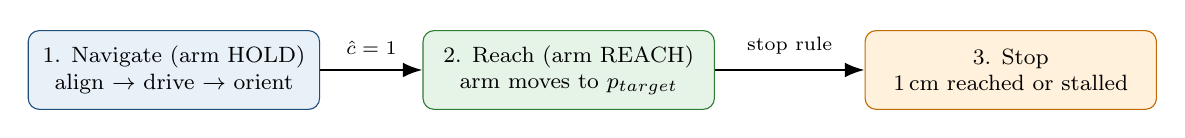
\begin{tikzpicture}[
  ph/.style={draw, rounded corners, align=center, minimum height=1.0cm, minimum width=3.7cm, font=\footnotesize},
  arr/.style={-{Latex[length=2.5mm]}, thick}]
\node[ph, fill=dagblueL, draw=dagblue] (a) {1. Navigate (arm HOLD)\\align $\to$ drive $\to$ orient};
\node[ph, fill=daggreenL, draw=daggreen, right=1.3cm of a] (b) {2. Reach (arm REACH)\\arm moves to $p_{target}$};
\node[ph, fill=dagorangeL, draw=dagorange, right=1.9cm of b] (c) {3. Stop\\1\,cm reached or stalled};
\draw[arr] (a)--(b) node[midway,above=2pt,font=\scriptsize]{$\hat c=1$};
\draw[arr] (b)--(c) node[midway,above=2pt,font=\scriptsize]{stop rule};
\end{tikzpicture}
\caption{Task phases and the network used in each. The latched flag $\hat c$ (Eq.~\eqref{dag:latch}) switches the arm from HOLD to REACH.}
\label{dag:phases}
\end{figure*}

During \emph{data collection} a rollout ends as soon as the end-effector has stayed within 5\,cm of the target for 30 consecutive steps. Rows beyond that point add little information. For the \emph{evaluation} the stop rule of the linear model's test is used unchanged (Section~\ref{sec:results}). The episode stops once the error is below 1\,cm (after at least 1\,s, with navigation done), or when the error has not improved by 2\,mm for 1.5\,s (``stalled''), or after 40\,000 steps (40\,s). Success means a \emph{final} error of at most 5\,cm. Two safety guards also end an episode as a failure: a joint angle above 15\,rad or a joint speed above 8\,rad/s.

\subsubsection{How the Final Version Was Reached}
\label{dag:history}

V6 was reached by trial and error. Each version fixed the main failure of the previous one, and the lessons are summarised here:
\begin{itemize}
  \item \textbf{V2: behaviour cloning.} One wheel MLP and one arm-torque MLP trained on the 38 raw world-frame features. A single arm network has to fit both the hold and the reach regime (Problem~1 of Section~\ref{sec:analysis}).
  \item \textbf{V4: phase-gated arm.} Separate HOLD/REACH arm networks selected by the navigation flag, and a joint-state history (lags of 10 and 30 \emph{rows}) to expose the expert's hidden reference. Still pure behaviour cloning, so the arm's errors were never corrected on the states it reached by itself.
  \item \textbf{V5 and V5.3: arm DAgger.} Two DAgger rounds on the arm (first $\beta=0.5$, then $\beta=0$), with the expert driving the wheels and the targets of the demonstrations. On those targets the policy reached 93.3\%. However, it reached only 6\% of tasks when the robot started up to 2\,m away. Most of these episodes ended in the velocity guard, after the base had driven into regions of the floor never seen in training.
  \item \textbf{V5.4: random targets, arm only.} A third arm round on 1400 random-target rollouts did \emph{not} help: these rollouts outnumbered the 161 earlier rollouts by 9:1, the fit moved away from the deployment distribution, and the wheel network was still never corrected.
  \item \textbf{V6: diagnosis and redesign.} Five causes were identified, each with a fix: (i)~demonstrations only from spawns within $\pm0.25$\,m and only 8\,s long $\Rightarrow$ DAgger rollouts from spawns in a $4\times4$\,m square, up to 60\,s; (ii)~a wheel network that was never DAgger-trained $\Rightarrow$ wheels mixed and learner-driven in rounds 1--2; (iii)~absolute world coordinates $\Rightarrow$ egocentric features \eqref{dag:ego}; (iv)~history lags defined in rows, which meant 100/300\,ms in the 10\,ms demonstrations but 10/30\,ms at deployment $\Rightarrow$ lags in seconds and 10\,ms resampling; (v)~a 20\,s step cap and a 25\,s navigation timeout that cut long drives short $\Rightarrow$ 60\,s and 45\,s. Lesson~(V5.4) also led to the per-episode row cap and the roughly 1:1 balance of demonstrations and rollouts.
\end{itemize}

\subsubsection{Closed-Loop Evaluation}
\label{dag:results}

\paragraph{Protocol} The policy was evaluated on \emph{the same 1000 episodes} as the linear model: the cases are regenerated with the random-number sequence and seed of the linear test script (\texttt{make\_linear\_protocol\_cases.py}). The base spawns uniformly in $x,y\in[-2,2]$\,m with a random heading, and the target is placed 0.9--3.5\,m from the spawn in a random direction, at a height of 0.3--0.9\,m. The stop rule and the success criterion are those of Section~\ref{dag:task}, with learner wheels and learner arm and no expert involvement. Two differences remain. The base goal is the expert's standoff pose \eqref{dag:goalpose}, which the policy was trained to imitate, rather than the linear model's spawn-bearing goal. In addition, the safety guards stay active and count as failures. The test distribution is also wider than the training distribution. Targets lie up to 6.1\,m from the world origin, and 76\% of them lie beyond the 1.8\,m training radius. This generalisation relies on the egocentric inputs.

\begin{table}[t]
\caption{Closed-Loop Results of the DAgger Policy (V6) on the 1000-Episode Linear-Model Protocol}
\label{dag:tab:results}
\centering
\footnotesize
\renewcommand{\arraystretch}{1.12}
\begin{tabular}{@{}lc@{}}
\toprule
\textbf{Metric} & \textbf{DAgger MLP (V6)}\\
\midrule
Success rate ($\le 5$\,cm) & 90.0\,\% (900/1000)\\
95\,\% Wilson interval & [88.0, 91.7]\,\%\\
Strict success ($\le 2$\,cm) & 56.5\,\%\\
Within 1\,cm & 19.6\,\%\\
Average / median final error & 79.0 / 18.0\,mm\\
Average / max error of successes & 18.5 / 49.9\,mm\\
Max error (all episodes) & 1.56\,m\\
Mean episode time (successes) & 14.2\,s\\
Stops: reached 1\,cm / stalled / step cap / guard & 196 / 731 / 73 / 0\\
Inference time / step (CPU) & 0.21\,ms\\
\bottomrule
\end{tabular}
\end{table}

\begin{figure}[t]
\centering
\includegraphics[width=0.75\linewidth]{\dagfigdir v6_dagger_rounds.pdf}
\caption{Closed-loop success of the checkpoint produced by each DAgger round on the first 200 episodes of the protocol, with 95\% Wilson intervals.}
\label{dag:fig:rounds}
\end{figure}

\begin{figure}[t]
\centering
\includegraphics[width=0.8\linewidth]{\dagfigdir v6_final_error_cdf.pdf}
\caption{Cumulative distribution of the final end-effector error over the 1000 episodes (log scale), with the fraction of episodes within 1, 2 and 5\,cm.}
\label{dag:fig:cdf}
\end{figure}

\begin{figure*}[t]
\centering
\includegraphics[width=0.85\linewidth]{\dagfigdir v6_success_map.pdf}
\caption{(a) Every target in the robot's initial body frame (the robot faces up), coloured by outcome; targets behind the robot require a turn before driving. (b) Success rate against the spawn--target distance, with 95\% Wilson intervals.}
\label{dag:fig:map}
\end{figure*}

\begin{figure*}[t]
\centering
\includegraphics[width=0.85\linewidth]{\dagfigdir v6_example_episodes.pdf}
\caption{Three example episodes driven entirely by the learned policy. (a) Top view of the base path from the spawn (dot) to the base goal (square); the star marks the target's $(x,y)$. (b) End-effector error over time; the dotted line marks the moment navigation completes and the REACH network takes over.}
\label{dag:fig:examples}
\end{figure*}

\paragraph{Results} Table~\ref{dag:tab:results} summarises the 1000 episodes. The policy reaches 900 targets (90.0\%, 95\% interval [88.0, 91.7]\%) from arbitrary spawn poses, with no expert involvement and no episode ended by a safety guard. Successful episodes finish on average 18.5\,mm from the target (at most 49.9\,mm). 19.6\% of all episodes stop at the 1\,cm criterion, and most of the others stop when the error stalls between 1 and 5\,cm (Fig.~\ref{dag:fig:cdf}). Fig.~\ref{dag:fig:examples} shows three typical episodes: the base turns toward its goal, drives, turns to the final heading, and then the REACH network takes the end-effector from tens of centimetres to under 5\,cm in about 2\,s.

\paragraph{Effect of DAgger} Fig.~\ref{dag:fig:rounds} compares the checkpoint of each round on the same 200 episodes. After round~0, which is pure behaviour cloning on the demonstrations plus expert-driven wide-spawn rollouts, the policy reaches \emph{none} of the 200 targets. Every episode ends in the joint-velocity guard. This is the compounding-error failure described in Section~\ref{dag:problem}: the networks' first small errors lead to states without training data, where the predicted torques diverge. A single round in which the learner controls half of the time raises the success rate to 89.5\% (179/200). The final $\beta=0$ round reaches 90.0\% (180/200) and removes the remaining safety-guard stops (6 in round~1, none in round~2).

\paragraph{Generalisation} Success does not drop outside the training region. Targets beyond the 1.8\,m training radius are reached in 90.9\% of episodes (686/755), and those inside it in 87.3\% (214/245), as expected from the translation-invariant inputs. Low targets ($z\le0.45$\,m), which need the elbow-twist branch of Problem~4 in Section~\ref{sec:analysis}, are somewhat harder: 82.6\% versus 92.6\% for higher targets.

\paragraph{Failure modes} The failures concentrate where the spawn lies \emph{close} to the base goal (Fig.~\ref{dag:fig:map}). Within 1\,m of it, the success rate is 52.3\% (81/155); beyond 1\,m it is 96.9\% (819/845). 73 of the 100 failures hit the 40\,s step cap, 62 of them with the spawn within 1\,m of the goal. Replays of these episodes show that the base does get within 7--8\,cm of its goal point, but still 1.0--1.5\,rad from the final heading. Instead of turning in place (the expert's \emph{orient} phase), it drives on and circles, so the navigation flag \eqref{dag:nav} is never set and the arm never starts reaching. Close to the goal the expert switches rapidly between its phases (align, short drive, passed-goal shortcut, orient), which is the least smooth part of its behaviour and the hardest for a regression network to imitate. The remaining 27 failures stall with the end-effector just outside the tolerance (median 7.0\,cm). The 300 test demonstrations remain untouched.

% -------------------------------------------------------------------------
% SUBSECTION C: RANDOM FOREST
% -------------------------------------------------------------------------
\subsection{Approach 3: Random Forest Controller}
\label{sec:rf}

The third approach uses a random forest base controller with goal-relative input features, paired with either a random forest arm or a DAgger-trained MLP arm (the V5.3 arm checkpoint of Section~\ref{dag:history}). On 100 held-out targets, the random forest base with the DAgger MLP arm succeeds in 97\% of trials within 5\,cm (34\% within 1\,cm), while the fully random forest controller fails in every trial despite an offline $R^2$ of up to 0.95.

\todo{Describe the random forest features, hyperparameters, training data and evaluation protocol, and explain why a high offline $R^2$ did not translate into closed-loop success.}

% =========================================================================
% SECTION IV: EXPERIMENTAL RESULTS
% =========================================================================
\section{Experiments and Results}
\label{sec:results}

\subsection{Test Protocol for the Linear Model}
To test whether the linear model generalises rather than memorising the training scenarios, a parallel evaluation script ran \textbf{1,000 new random episodes} with:
\begin{itemize}
    \item a random base starting position shifted by up to $\pm 0.25\,\text{m}$;
    \item a random initial heading over the full $360^\circ$ ($-\pi$ to $+\pi$);
    \item random 3D targets between $0.9\,\text{m}$ and $3.5\,\text{m}$ away, at heights from $0.3\,\text{m}$ to $0.9\,\text{m}$;
    \item random initial arm joint perturbations of up to $\pm 0.1\,\text{rad}$.
\end{itemize}
A trial counts as a success if the gripper gets within $0.05\,\text{m}$ of the target within 20\,s.

\begin{figure}[t]
\centering
\includegraphics[width=\columnwidth]{figures/failure_5_random_test_fixes.png}
\caption{Why the base stopped at the wrong distance. The robot approaches from outside the stop window. With a wide window ($0.60 \le t_f \le 0.82$\,m) it always stopped prematurely at the outer edge ($0.82$\,m). Targeting the arm's sweet spot ($t_f \approx 0.705$\,m) and tracking the bearing live raised the 1,000-trial success rate from 45.2\% to 100.0\%.}
\label{fig:sweet_spot}
\end{figure}

\subsection{The Sweet-Spot Parking Fix}
In the first run of 1,000 episodes the success rate was only $45.2\%$, with errors peaking at $5.2\,\text{cm}$. Inspection of the data revealed two causes (Fig.~\ref{fig:sweet_spot}):
\begin{enumerate}
    \item \textbf{Stopping at the outer edge:} because the robot approaches the target from outside, a wide stop window ($0.60 \le t_f \le 0.82\,\text{m}$) always triggered as soon as the robot crossed the outer boundary ($t_f = 0.82\,\text{m}$), leaving the arm reaching at the edge of its workspace.
    \item \textbf{Skid-steer drift:} turning in place on four wheels shifted the base sideways by $6$--$9\,\text{cm}$.
\end{enumerate}
Both were fixed by stopping at the arm's sweet spot ($t_f^{\text{ideal}} = \text{standoff} + 0.055 \approx 0.705\,\text{m}$) and tracking the target bearing live. This shifted the error distribution close to zero and raised the success rate to $100\%$.

\subsection{Comparison of the Approaches}
Table~\ref{tab:comparison} compares the linear model and the DAgger MLP on \emph{the same} 1,000 randomised test episodes, with the same stop rule and success criterion (Section~\ref{dag:results}). The random forest results of Section~\ref{sec:rf} were obtained on a different protocol (100 held-out targets) and are not included.

\begin{table}[t]
\caption{Performance of the Decoupled Linear Model and the DAgger MLP on the Same 1,000 Random Episodes}
\label{tab:comparison}
\centering
\begin{tabular}{@{}lcc@{}}
\toprule
\textbf{Metric} & \textbf{Linear Reg.} & \textbf{DAgger MLP} \\
\midrule
Total parameters & 246 & 342\,674 \\
Training time & 1.8\,s & 44\,min$^\ddagger$ \\
Inference time / step & 0.03\,ms & 0.21\,ms \\
Success rate ($\le 5\,\text{cm}$) & 100.0\% & 90.0\% \\
Strict success ($\le 2\,\text{cm}$) & 94.5\% & 56.5\% \\
Average error$^\dagger$ & 6.3\,mm & 79.0\,mm \\
Median error$^\dagger$ & 3.8\,mm & 18.0\,mm \\
Max error$^\dagger$ & 31.8\,mm & 1.56\,m \\
\bottomrule
\multicolumn{3}{@{}p{0.95\columnwidth}@{}}{\footnotesize $^\dagger$Final end-effector error over all 1,000 episodes, failures included. $^\ddagger$Final DAgger round on a GTX~1650 GPU; the full pipeline, including 1,600 simulated rollouts, takes about 3.2\,h.}
\end{tabular}
\end{table}

\subsection{Discussion}
Why does a simple linear model perform so well on this task?
\begin{itemize}
    \item \textbf{No training hyperparameters:} linear regression has no learning rate, batch size or local minima. The optimal weights are obtained in a single closed-form step ($\mathbf{W} = \mathbf{X}^+ \mathbf{Y}$) in under 2 seconds.
    \item \textbf{Stability by construction:} removing collinear features and using body-frame inputs removes the mechanism that produced the positive-feedback instability, and the learned joint stiffnesses are all negative.
    \item \textbf{Speed:} with only 246 parameters, inference is a single matrix--vector product taking $0.03\,\text{ms}$ on a standard CPU.
\end{itemize}
The cost is that this performance depends on extensive hand-engineered features and a hand-designed parking rule. The DAgger MLP uses only a generic egocentric transform and learns the whole controller from data, including recovery from its own errors. It drives the full distance itself and generalises to targets outside its training region. In exchange it needs about 1,400 times more parameters and hours of simulated rollouts, and it is less precise (median 18.0\,mm versus 3.8\,mm). One reason is that its rollouts end 30\,ms after entering the 5\,cm band, so few training rows show the final convergence. The linear base also stops at a sweet spot measured on the target itself, whereas the MLP imitates the expert's standoff goal; the MLP's remaining failures are short-range base manoeuvres near that goal (Section~\ref{dag:results}).

% =========================================================================
% SECTION V: CONCLUSION & FUTURE WORK
% =========================================================================
\section{Conclusion and Future Work}
\label{sec:conclusion}

\subsection{Summary}
This project showed that mobile manipulation by behaviour cloning does not necessarily require large neural networks. By analysing why naive learning failed (regime mixing, world-coordinate sign flips, anti-spring feedback and elbow-twist branching), a decoupled linear regression model was designed that reached 3D targets with $100\%$ success and millimetre-level accuracy across 1,000 random test trials. The DAgger-trained MLP policy, using only a generic egocentric feature transform, reached 90.0\% success on the same 1,000 trials from arbitrary spawn poses; an earlier version of its arm, combined with a random forest base, succeeded in 97\% of 100 held-out trials.

\subsection{Limitations: What About Clutter?}
\label{sec:limitations}
The models assume an open room with a direct line of sight to the target. If chairs, tables or walls were in the way:
\begin{itemize}
    \item the base models would drive straight into them, because they have no sensors to detect obstacles;
    \item \textbf{future work:} in a cluttered room the robot would need a 2D/3D LiDAR or a depth camera. A global planner (such as $A^*$, RRT$^*$ or the ROS2 Nav2 stack we experimented with) would find an obstacle-free path, and the learned base model would track its waypoints one by one as a local planner.
\end{itemize}

% =========================================================================
% REFERENCES
% =========================================================================
\begin{thebibliography}{00}

\bibitem{siegwart2011autonomous}
R.~Siegwart, I.~R.~Nourbakhsh, and D.~Scaramuzza, \textit{Introduction to Autonomous Mobile Robots}, 2nd~ed. Cambridge, MA, USA: MIT Press, 2011.

\bibitem{coumans2016pybullet}
E.~Coumans and Y.~Bai, ``PyBullet, a Python module for physics simulation for games, robotics and machine learning,'' \textit{GitHub repository}, 2016.

\bibitem{laskey2017dart}
M.~Laskey, J.~Lee, R.~Fox, A.~Dragan, and K.~Goldberg, ``DART: Noise injection for robust imitation learning,'' in \textit{Proc. 1st Conf. Robot Learn. (CoRL)}, PMLR 78, pp. 143--156, 2017.

\bibitem{takegaki1981new}
M.~Takegaki and S.~Arimoto, ``A new feedback method for dynamic control of manipulators,'' \textit{ASME J. Dyn. Syst., Meas., Control}, vol. 103, no. 2, pp. 119--125, 1981.

\bibitem{bishop1994mixture}
C.~M.~Bishop, ``Mixture density networks,'' Neural Computing Research Group, Aston University, Tech. Rep. NCRG/94/004, 1994.

\bibitem{ross2011reduction}
S.~Ross, G.~J.~Gordon, and J.~A.~Bagnell, ``A reduction of imitation learning and structured prediction to no-regret online learning,'' in \textit{Proc. 14th Int. Conf. Artif. Intell. Statist. (AISTATS)}, PMLR 15, pp. 627--635, 2011.

\end{thebibliography}

% =========================================================================
% AUTHOR CONTRIBUTION STATEMENT
% =========================================================================
\clearpage
\onecolumn
\section*{Author Contribution Statement}

Per the COMP0245 submission guidelines, the contributions of each group member are summarised below.

\vspace{0.5cm}
\begin{itemize}
    \item \textbf{Shivansh Chaudhary (Linear Regression Lead, Data Analysis and Diagnostics):}
    \begin{itemize}
        \item Conducted the exploratory data analysis and diagnosed the four root causes of naive imitation failure (regime mixing, world-coordinate sign flips, anti-spring positive feedback and elbow-twist branching).
        \item Formulated the body-frame ($SO(2)$ rotation) coordinate transformations that fix the rotational non-invariance.
        \item Built the decoupled 15-feature base navigation model with distance saturation and alignment gating (\texttt{drive\_term}).
        \item Built the 25-feature arm torque model using DART state perturbation to learn the stabilising PD spring stiffness ($-100$\,N$\cdot$m/rad) and gravity compensation.
        \item Identified the sweet-spot base parking condition and live bearing tracking, and implemented the 1,000-trial parallel evaluation suite.
        \item Authored Section~\ref{sec:analysis} (Data Analysis), Section~\ref{sec:linear} (Linear Regression Methodology), Section~\ref{sec:results} (Experiments and Results) and Section~\ref{sec:conclusion} (Conclusion and Limitations).
    \end{itemize}

    \vspace{0.4cm}
    \item \textbf{Ricktho Sarkar (MLP Policy and DAgger):}
    \begin{itemize}
        \item Designed the PyTorch MLP policy (wheel network and phase-gated HOLD/REACH arm networks with time-based joint history) and the egocentric feature representation.
        \item Implemented the DAgger pipeline: the collector that advances the stateful expert on every learner state, $\beta$-mixing of wheels and arm, parallel resumable rollouts, data aggregation and the training script.
        \item Iterated the policy from behaviour cloning (V2) to the final V6, diagnosed the random-spawn failures of the earlier versions, and evaluated the final policy on the linear model's 1,000-episode protocol.
        \item Authored Section~\ref{dag:sec} (MLP Policy with DAgger) and the DAgger column of Table~\ref{tab:comparison}.
    \end{itemize}

    \vspace{0.4cm}
    \item \textbf{Hafizh Ilham (Random Forest Controller):}
    \begin{itemize}
        \item \todo{Summarise your specific contributions, e.g.\ feature design, hyperparameter tuning and evaluation of the random forest controllers.}
        \item Authored Section~\ref{sec:rf} (Random Forest Controller) and generated the corresponding metrics.
    \end{itemize}
\end{itemize}

\end{document}
